As mentioned in the report, the calculations in the variation of height are made considering that a Hohmann maneuver is applied. The main characteristics of this maneuver are explained on the following sections.

\subsubsection{Energy equation}
The deduction of the equations needed to solve the Hohmann maneuver begins with the energy equation:

\begin{equation}
\frac{V^2}{2}-\frac{\mu}{r}=-\frac{\mu}{2a}
\end{equation}
where $V$ is the orbital velocity of the satellite, $r$ is the distance from the focus, $a$ the semimajor axis of the orbit and $\mu$ the gravitational constant of the attracting body, in this case, the Earth. This expression shows that the total energy of the satellite equals the sum of its kinetic  and potential energy (per mass unit).

This equation can be arranged to obtain the velocity of the satellite. In the case of a circular orbit, the radius is constant, and equal to the semimajor axis. Replacing $a=r$ in the energy equation and after some operations, the expression of the velocity of a circular orbit is obtained:
\begin{equation}
V_{c}=\sqrt{\frac{\mu}{r}}
\end{equation}

As it can be deduced from the energy equation, a change in orbital velocity leads to a change in the value of the semimajor axis. This property is used in satellites to change their orbit through a velocity increment $\Delta V$. This process is called an orbital maneuver.

\subsubsection{Delta-V}
If the velocity increment $\Delta V$ is done instantaneously, the maneuver is called an impulsive maneuver. The Hohmann transfer is a two-impulse transfer between coplanar circular orbits. From an inicial circular orbit, a tangential velocity increment $\Delta V_{1}$ is applied to change the orbit to an ellipse. This ellipse is the transfer orbit, in which the perigee radius is the radius of the initial circular orbit and the apogee radius equals the radius of the final circular orbit. When the satellite reaches the apogee, a second velocity increment $\Delta V_{2}$ is applied, so that the satellite reaches the final circular orbit with the apogee radius. If this second velocity is not applied, the satellite will remain in the elliptic orbit.

\begin{figure}
\centerline{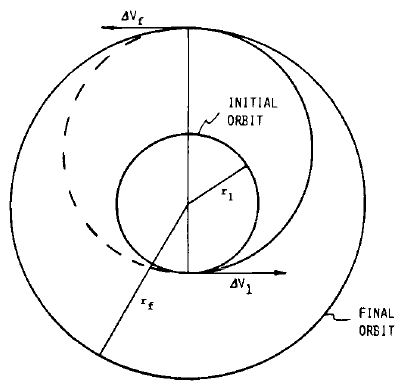
\includegraphics[scale=0.7]{Hohmann.png}}
\caption{Hohmann transfer. Extracted from \cite{Chobotov2002}}
\end{figure}

With the energy equation defined above, it is easy to determine the velocity of the satellite in each orbit. The first orbit and the final ones are circular:

\begin{equation}
V_{1}=\sqrt{\frac{\mu}{r_{1}}}
\end{equation}
\begin{equation}
V_{f}=\sqrt{\frac{\mu}{r_{f}}}
\end{equation}

The velocity in the transfer orbit can be easily calculated with the energy equation applying the definition of the semimajor axis of an ellipse:

\begin{equation}
a=\frac{r_{1}+r_{f}}{2}
\end{equation}
The velocities in the perigee and apogee are:
\begin{equation}
V_{p}=\sqrt{\frac{2\mu r_{f}}{r_{1}(r_{1}+r_{f})}}
\end{equation}
\begin{equation}
V_{a}=\sqrt{\frac{2\mu r_{1}}{r_{f}(r_{1}+r_{f})}}
\end{equation}
Therefore the velocity increments are:
\begin{equation}
\Delta V_{1}=V_{p}-V_{1}=\sqrt{\frac{2\mu r_{f}}{r_{1}(r_{1}+r_{f})}}-\sqrt{\frac{\mu}{r_{1}}}
\end{equation}
\begin{equation}
\Delta V_{2}=V_{f}-V_{a}=\sqrt{\frac{\mu}{r_{f}}}-\sqrt{\frac{2\mu r_{1}}{r_{f}(r_{1}+r_{f})}}
\end{equation}

\subsubsection{Time}
It is also necessary to know the time needed to do the maneuver. This time is equal to half of the period of the transfer ellipse:
\begin{equation}
t=\frac{T}{2}=\frac{1}{2}\sqrt{\frac{4\pi^{2}a^{3}}{\mu}}
\end{equation}

\subsubsection{Propellant}
In order to know the mass of propellant needed in the maneuver, the Tsiolkovsky rocket equation is applied:
\begin{equation}
\Delta V=g_{0}I_{sp}\ln{\frac{m_{1}}{m_{f}}}=g_{0}I_{sp}\ln{\frac{m_{1}}{m_{1}-m_{prop}}}
\end{equation}
where $\Delta V=\Delta V_{1}+\Delta V_{2}$ is the total velocity increment of the maneuver, $g_{0}$ is the Earth's gravity, $I_{sp}$ is the specific impulse of the thruster used, $m_{1}$ is the initial mass of the satellite, $m_{f}$ is its final mass and $m_{prop}$ is the mass of propellant used in the maneuver.
\begin{equation}
m_{prop}=m_{1}\Bigg(1-\exp\bigg(-\frac{\Delta V}{g_{0}I_{sp}}\bigg)\Bigg)
\end{equation}